\documentclass{article}

% Language setting
% Replace `english' with e.g. `spanish' to change the document language
\usepackage[danish]{babel}
% Set page size and margins
% Replace `letterpaper' with `a4paper' for UK/EU standard size
\usepackage[a4paper,top=2cm,bottom=2cm,left=3cm,right=3cm,marginparwidth=1.75cm]{geometry}

% Useful packages
\usepackage{amsmath}
\usepackage{graphicx}
\usepackage[colorlinks=true, allcolors=blue]{hyperref}
\usepackage{array}
\usepackage{subfig}
\usepackage{subfigure}
\usepackage{titlesec}
\usepackage{enumitem}

\title{CDIO delopgave 0}
\author{Jakob Agergaard}
\linespread{1.25}


\begin{document}

\titlespacing{\section}
    {0pt}{2em}{1em}




\begin{titlepage}
\begin{center}

    
\includegraphics[width=0.25\textwidth]{Billeder/DTULogo.png} \\
    \vspace{0.5cm}
    \Large
    \textbf{02314\hspace{1cm}62531\hspace{1cm}62532} \\
    Indledende programmering, Udviklingsmetoder til IT-systemer og Versionsstyring og testmetoder
    \vspace{0.4cm}
    \hrule
    
    \vspace*{0.5cm}
    \huge
    \textbf{CDIO delopgave 0}\\
    \LARGE
    Gruppe 17
    \vspace{0.5cm}
    \hrule
    \vspace{0.2cm}

    \large
    \begin{tabular}{m{10em} m{8em} m{8em} m{10em}}
    Jakob Skov Agergaard\vfill s224570 & 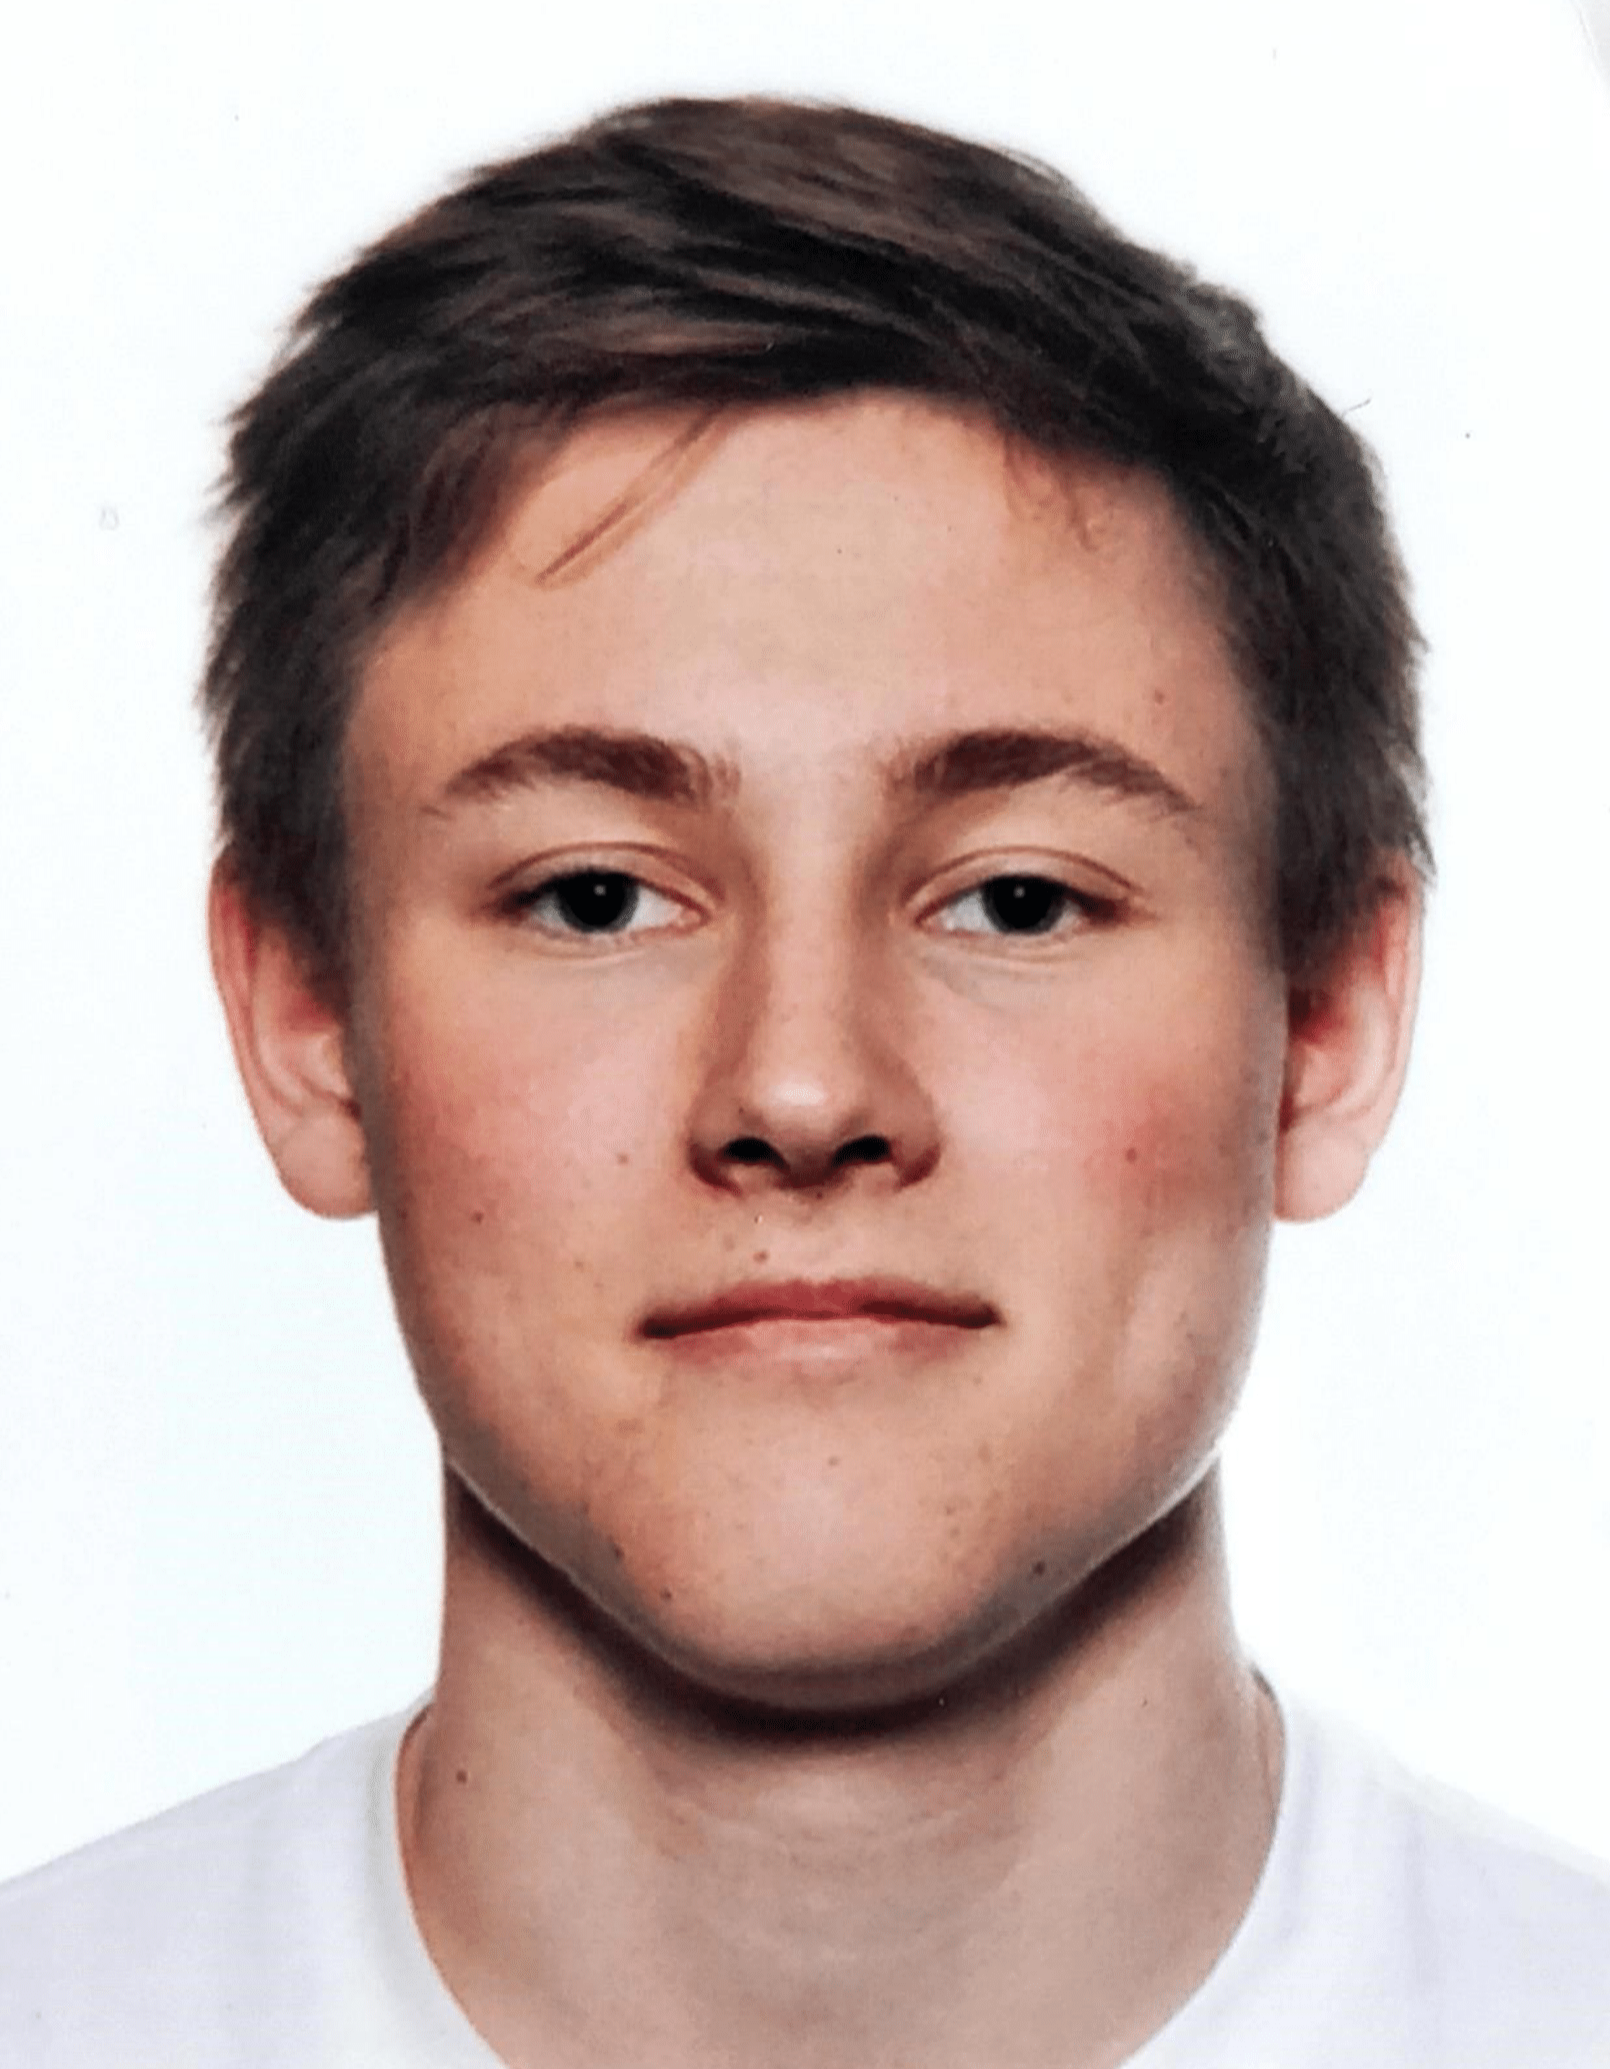
\includegraphics[width=0.2\textwidth]{Billeder/JakobFoto.png} & 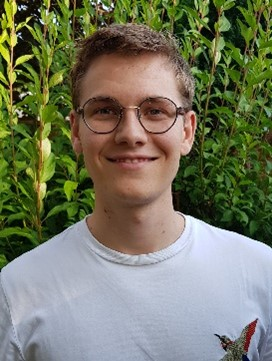
\includegraphics[width=0.2\textwidth]{Billeder/PhilipFoto.jpg} & Philip Muff Førrisdahl\vfill s224566 \\
    Mads Fogelberg Hansen\vfill s224563 & 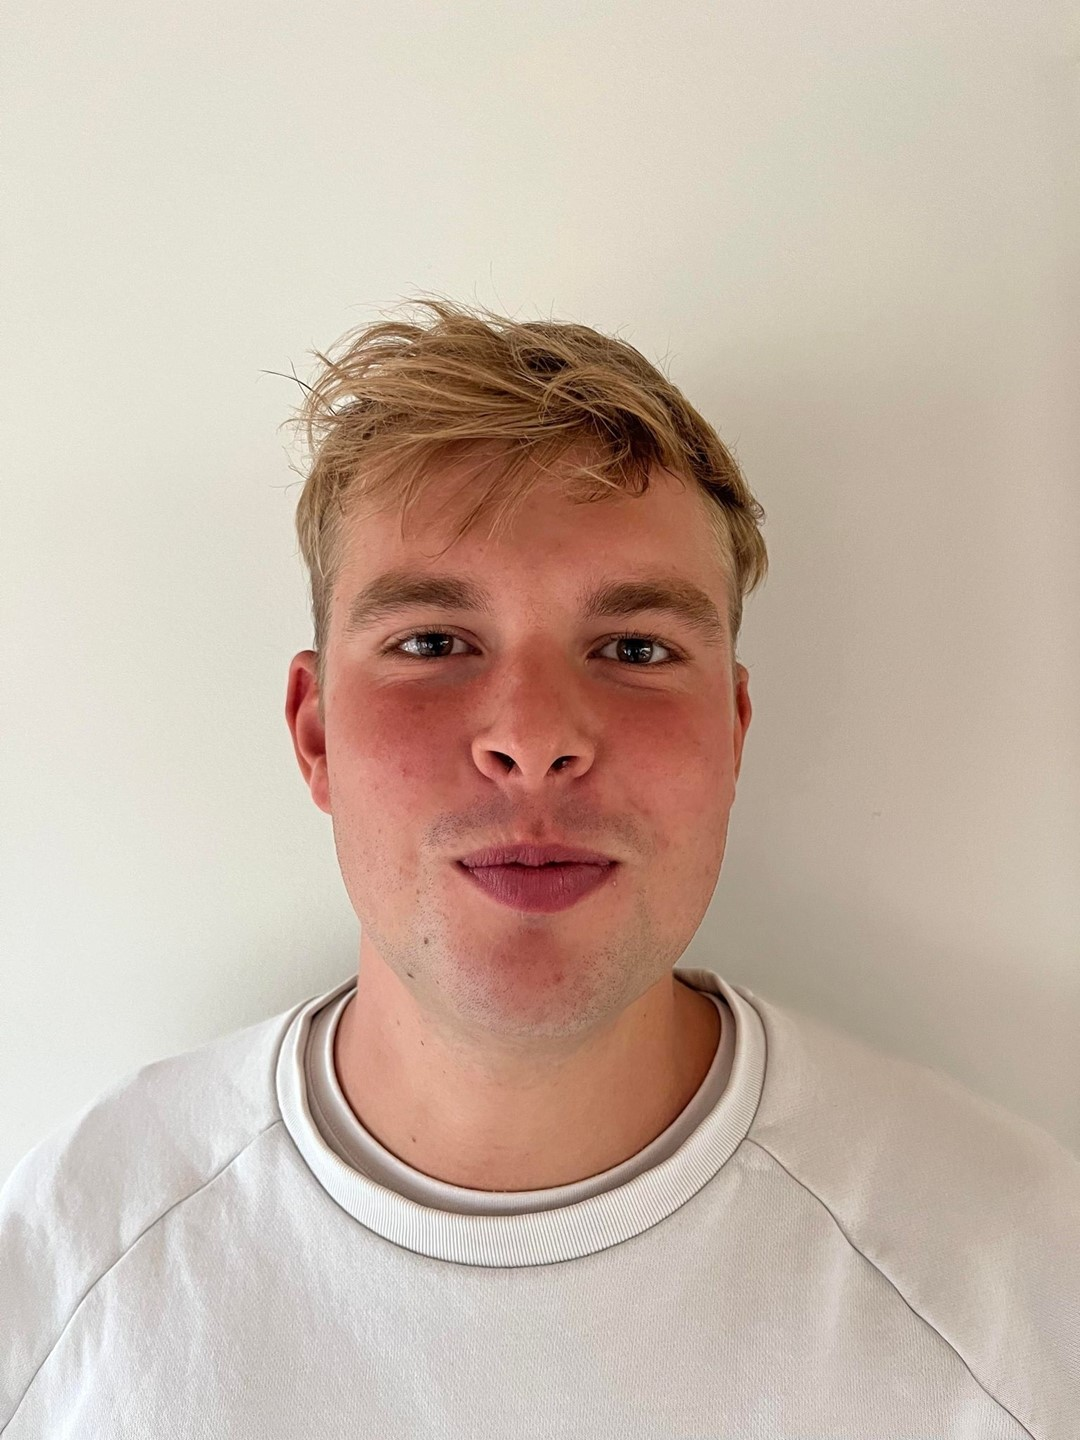
\includegraphics[width=0.2\textwidth]{Billeder/FotoMads.jpg} & 
\includegraphics[width=0.2\textwidth]{Billeder/EsbenFoto.png} & Esben Skovmand Elnegaard \vfill s224555  \\
    Jarl Boyd Roest\vfill s224556 & 
\includegraphics[width=0.2\textwidth]{Billeder/JarlFoto.png}
    \end{tabular}

    \vfill
    
    
    \vspace{1cm}
    \LARGE
    18. september 2022

    \vspace{1cm}
    
\end{center}
\end{titlepage}


\normalsize
\begin{abstract}
This report documents our process in the making of Monopoly Junior. Our product of the game has been produced partly by the costumers vision and partly on the prioritesed list of requirements/rules that we made at the start of the project.
This report documents the initial analysis of the problem, the requiremts analysis, the design of the game in form of different diagrams, other artifacts and our different tests.


\end{abstract}
\break 

\tableofcontents
\break 

\section{Timeregnskab}
\begin{itemize}
    \item Arbejdsdag 1: 2 timer
    \item Arbejdsdag 2: 1.5 timer
    \item Arbejdsdag 3: 1.5 timer
    \item Arbejdsdag 4: 2 timer
    \item Arbejdsdag 5: 2.5 timer
    \item Arbejdsdag 6: 4 timer
    \item Arbejdsdag 7: 1.5 timer 
    \item Arbejdsdag 8: 3 timer
    \item Arbejdsdag 9: 2 timer
    \item Arbejdsdag 10: 2 timer
    \item Arbejdsdag 11: 2 timer
\end{itemize}
\section{Indledning}
I følgende rapport bliver hele handlingsforløbet af vores CDIO-3 projekt beskrevet, samt dokumentation af denne proces. Rapporten giver kendskab til udviklingsmetoderne, som er brugt i processen. Projektet tager udgangspunkt i børnespillet Monopoly Junior, men med mulighed for at implementere eller tilføje relevante ting. Der har været fokus på at bruge Rational Unified Process, som derfor har ført til små iterationer, evalueringer og opsamlinger under hele forløbet, både på forarbejdet og under programmerings delen, for hele tiden at sikre os at programmet kører som det skulle. Derudover er der blevet produceret en række diagrammer, som har overskueliggjort opgaven. Der har været fokus på at bruge Low Coupling og High Cohesion til at lave diagrammerne. Dette kan ses da der har været fokus på nedarvning i diagrammerne, så klasserne arver metoder og variabler fra hinanden. 

\section{Projekt-planlægning}
\begin{itemize}
    \item [1/11] I denne session arbejder vi på udfærdigelsen af opgaveprioritering og udarbejder en kravsliste over funktionelle krav.\\
    Evaluering på dagen: Alt nået
    \item [2/11] I denne session vil udarbejde en primær use case beskrivelse (brief) og identificere andre sub-use cases. Udarbejde et use case diagram og starte på domænemodel.\\
    Evaluering på dagen: Alt nået, samt domænemodel færdiggjort og start på designklasse diagrammet. Vi har implementeret de første og mest simple klasser i IntelliJ.
    \item [4/11] Denne dag skal der laves systemsekvensdiagram samt sekvensdiagram.
    \item [7/11]
    Afklaring af hvilke regler vi vil implementere og hvilke vi vil udelade, udover dem fra vores kravspecifikation. Design og test af boardclass og squareclass.
    \item [11/11]
    Opgaver for denne session:
    Færdiggjort strukturen af vores domæne/klassediagram. Få oprettet alle klasser samt toString metoder, samt toString metode til array. Oprettet og begynde små test i game class. Alt nået.
    
    \item [14/11]
    Opgaver løst: GUI implementeret. Game funktionalitet implementeret og  første version af spillet færdigt. 
    
    Opgaver til næste session: Implementere chancekort. Beskrivelse (output til spilleren) til felter og actions. Identificere test og test cases.
    
    \item[15/11]
            Gennemgang af hvad programmet mangler, hvilke opgaver der skal løses og i hvilken rækkefølge,  og uddelegering af opgaver til enkeltmand. * Se billede Plan Banan * 

\begin{figure} [h]
        \centering
            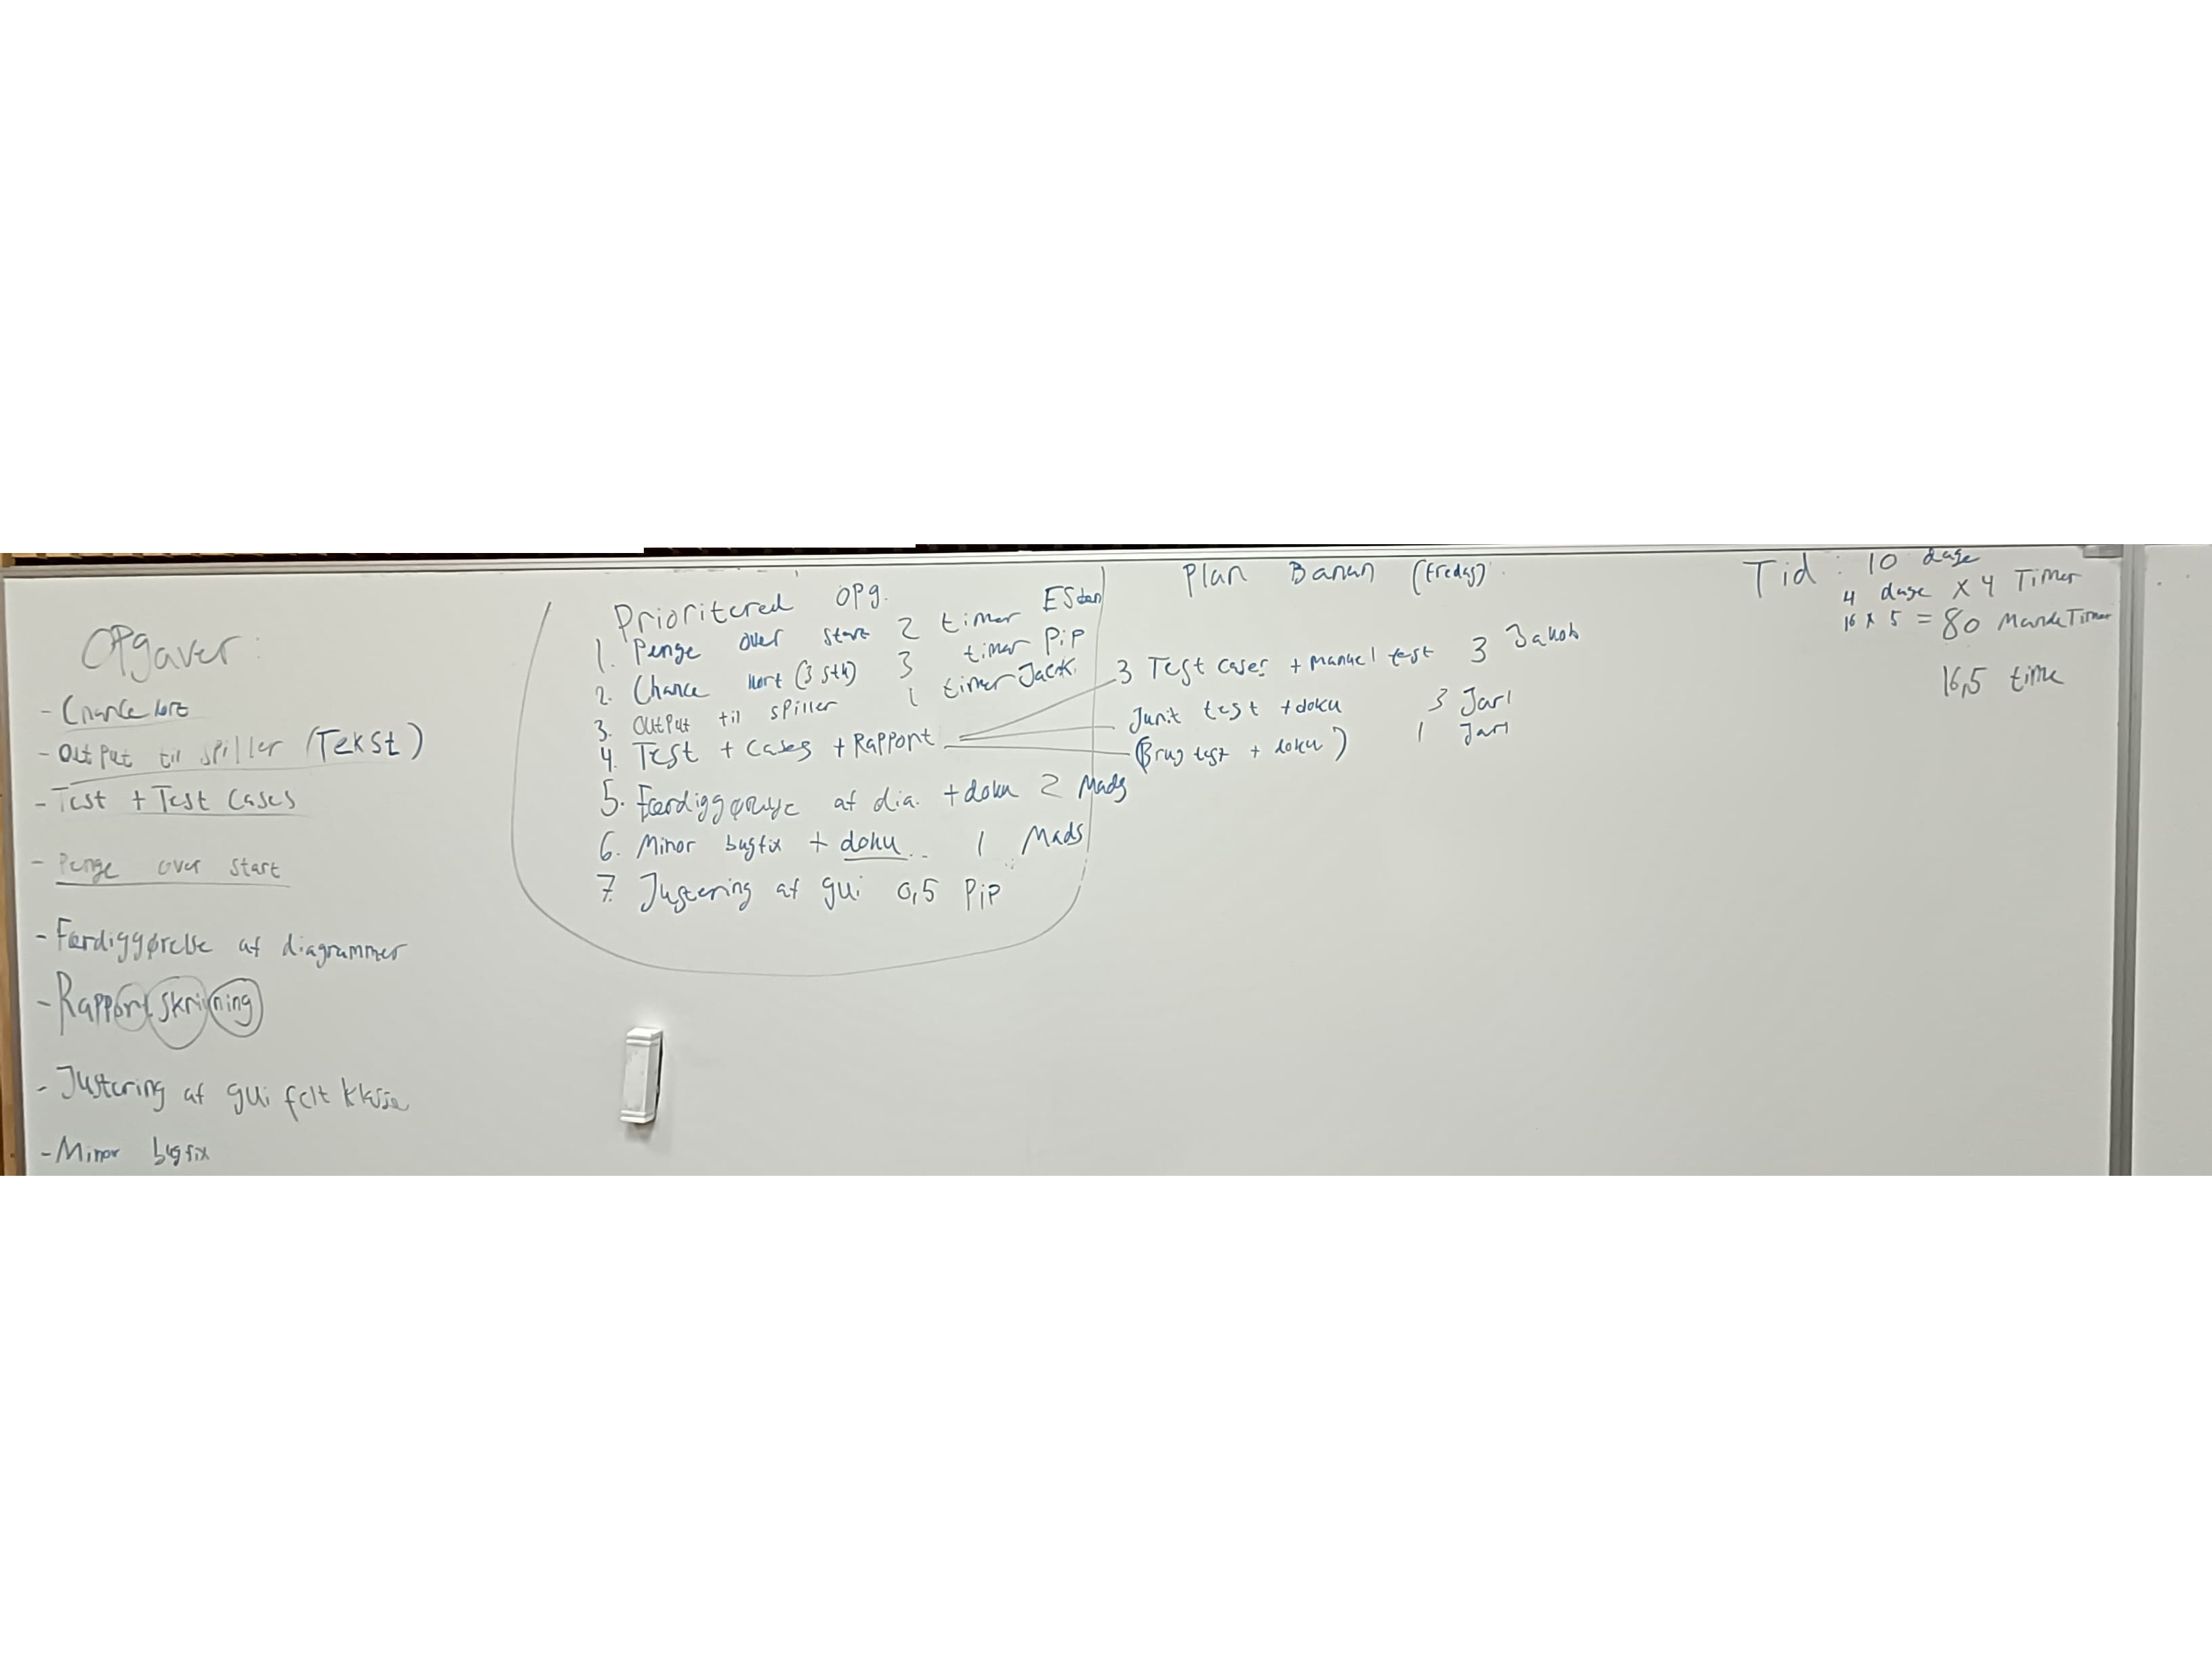
\includegraphics[width = 1.0
            \textwidth]{Billeder/planBanan.png}
            \caption{Plan Banan}
            \label{PlanBanan}
    \end{figure}
     
    \item[18/11]
            Folk laver tildelte opgaver, og en opsamling til sidst. 
            * Se billede Plan Banan*.
           
            Opsamling: Opgaver ikke nået; JUnittest, GUI-implementation af chancekort. Ansvarlige færdiggøres i weekend inden næste session.
                      
    \item [22/11]
    Sidste bugs vi har identificeret er løst, flere er dog identificeret men givet tiden til rådighed, vælger vi at lav code-freeze og fokusere på færdiggørelsen af rapporten. Den bliver skrevet færdig d. 25/11.
	\item[21/11]
    Gennemgang af de tildelte opgaver, og videre arbejde af dem, hvis der er mangler. Code Freeze
            
    \item[25/11]
    Rapporten skal færdiggøres og afleveres.
\end{itemize}

		
\section{Krav/Analyse}
\subsection{Kravsliste | funktionelle krav}
\begin{enumerate}
    \item Skal kunne spilles af 2-4 spillere (opfyldt)
    \item Spilleplade med 24 felter (opfyldt)
    \item Man skal kunne købe og derefter eje felter (opfyldt)
    \item Spillerne skal have hver deres egen pengebeholdning (opfyldt)
    \item Hvis én af spillernes pengebeholdning går i minus slutter spillet (opfyldt)
    \item En terning med seks sider (opfyldt)
    \item En brik per spiller, som kan rykke (opfyldt)
\end{enumerate}
\subsection{Prioritering af krav vi vil implementere, når de funktionelle krav er opfyldt}
\begin {itemize}
\item Vi implementerer 3 af chancekortenes funktioner. Hvis der er tid implementere vi flere slags chancekort. (implementeret)
\item Fængsel felt og funktion bliver ikke implementeret. I stedet bliver de felter 'NoActionsFields' (ej implementeret)
\item Man får ikke mulighed for at vælge bil/farve men får blot tildelt en i starten af spillet. (ej implementeret)
\item  Spilstarteren bliver  den spiller der først indtaster sit navn (implementeret)
\item Spillerne starter med et tilpasset antal penge alt efter antal spillere (implementeret)
\item Spillere modtager penge ved landing eller passering af 'Start'-felt (implementeret)
\item Hvis spilleren lander på et ledigt ejendeomsfelt, skal spillere købe det. Hvis spilleren lander på sit eget felt skal spilleren ikke gøre noget. Dobbelt-ejendomsfelt reglen er udeladt.(implementeret)
\item Hvis spilleren lander på en andens ejendomsfelt, skal spilleren betale husleje. (implementeret)
\item Hvis 2 spillere har den samme pengebeholdning, i slutningen af spillet bliver værdien af deres ejedoms også sammentalt for at finde en endelig vinder. (ej implementeret)
\end {itemize}
\subsection{Use case beskrivelse og analyse }
\textbf{Use case på 'brief format'}\\
Spillerene indtaster hvor mange spillere de er, og skriver derefter navnene på deres brikker som de vil have vist i spillet. Første spiller slår med ternigen, og rykker det antal øjne som terningen viser. Systemet udfører derefter handlingen for det pågældende felt som spilleren er landet på. Turen går derefter videre til næste spiller.
\\
\\
\textbf{Use case beskrevet på 'fully dressed' format}
\\
\textbf{Scope:} Spil Monopoly Junior 
\\
\textbf{Level:} Spillere
\\
\textbf{Primary actor:} Spillere 2 - 4 
\\
\textbf{Stakeholders and interests} 
\begin{itemize}
    \item Spillerne vil spille et underholdende spil med formål at vinde. 
    \item Projektvejlederen vil have et Monopoly Junior spil, som vil tilfredsstille kundens vision og krav
    \item Kunden vil have et monopolyspil, som har taget udgangspunkt i den fremlagte vision og de dertil hørende Monopoly Junior regler 
\end{itemize}
\\
\textbf{Preconditions:} Computeren, som skal køre Monopoly Junior skal have den nyeste version af Java. 
\\
\textbf{Succes guarantee:} Spilleren har slået med terningerne, rykket sine brikker og evt. købt/betalt/fået beløb, og turen er gået videre til næste spiller. 
\\
\\
\textbf{Main Scenario}
\begin{enumerate}
\itemsep-0.5em
    \item Første spiller slår med terningen
    \item Første spillers brik bliver nu rykket det antal felter som terningernes øjne viser.
    \item Spilleren lander på et felt og systemet fortæller hvilket felt man er landet på.
    \item Systemet fortæller hvilken handling eller hvad feltet gør\\
    \textit{Punkterne 1-5 bliver nu gentaget for næste spiller}
\end{enumerate}

\textbf{Extension (Alternate Succes Scenario): }
\begin{enumerate}
    \item [4.a] Spilleren lander på en grund der ikke er købt endnu. Systemet fortæller spilleren hvilket felt de er landet på. Spilleren har dog ikke nok penge til at betale feltets pris.
    \subitem 1. Spillet slutter da en spiller er gået fallit. Alle spillernes pengebeholdning bliver talt op, og den med flest penge vinder.
    \item [4.b] Spilleren lander på en grund der er købt. System fortæller spilleren hvilket felt de er landet på, og spilleren betaler samtidig husleje til spilleren som ejer feltet.
    \item [4.c] Spilleren lander på et felt uden handling.
\end{enumerate}

\begin{figure} [h]
    \centering
    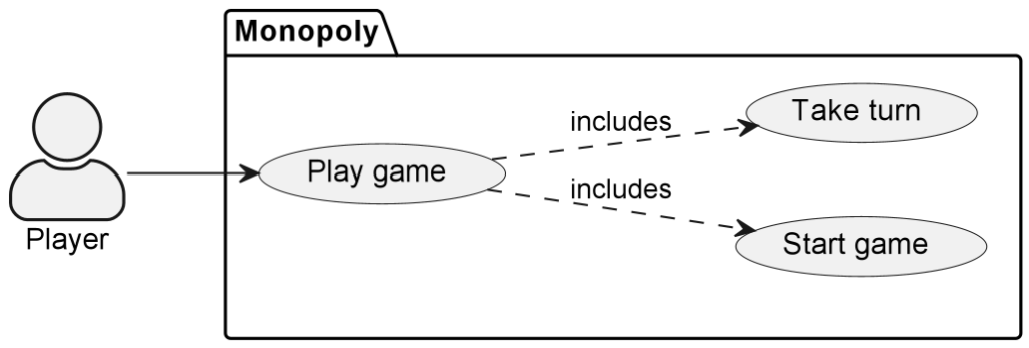
\includegraphics[width = 0.4\textwidth]{Billeder/Usecasediagram.png}
    \caption{Use case diagram}
    \label{Use case diagram}
\end{figure}
Dette use case diagram(Figur 2) viser hvordan spilleren og systemet interagere med hinanden. Spiller skal starte spillet og derefter starte turen, hvorefter spillet køre mere eller mindre ad sig selv. 
\\

\begin{figure} [h]
    \centering
    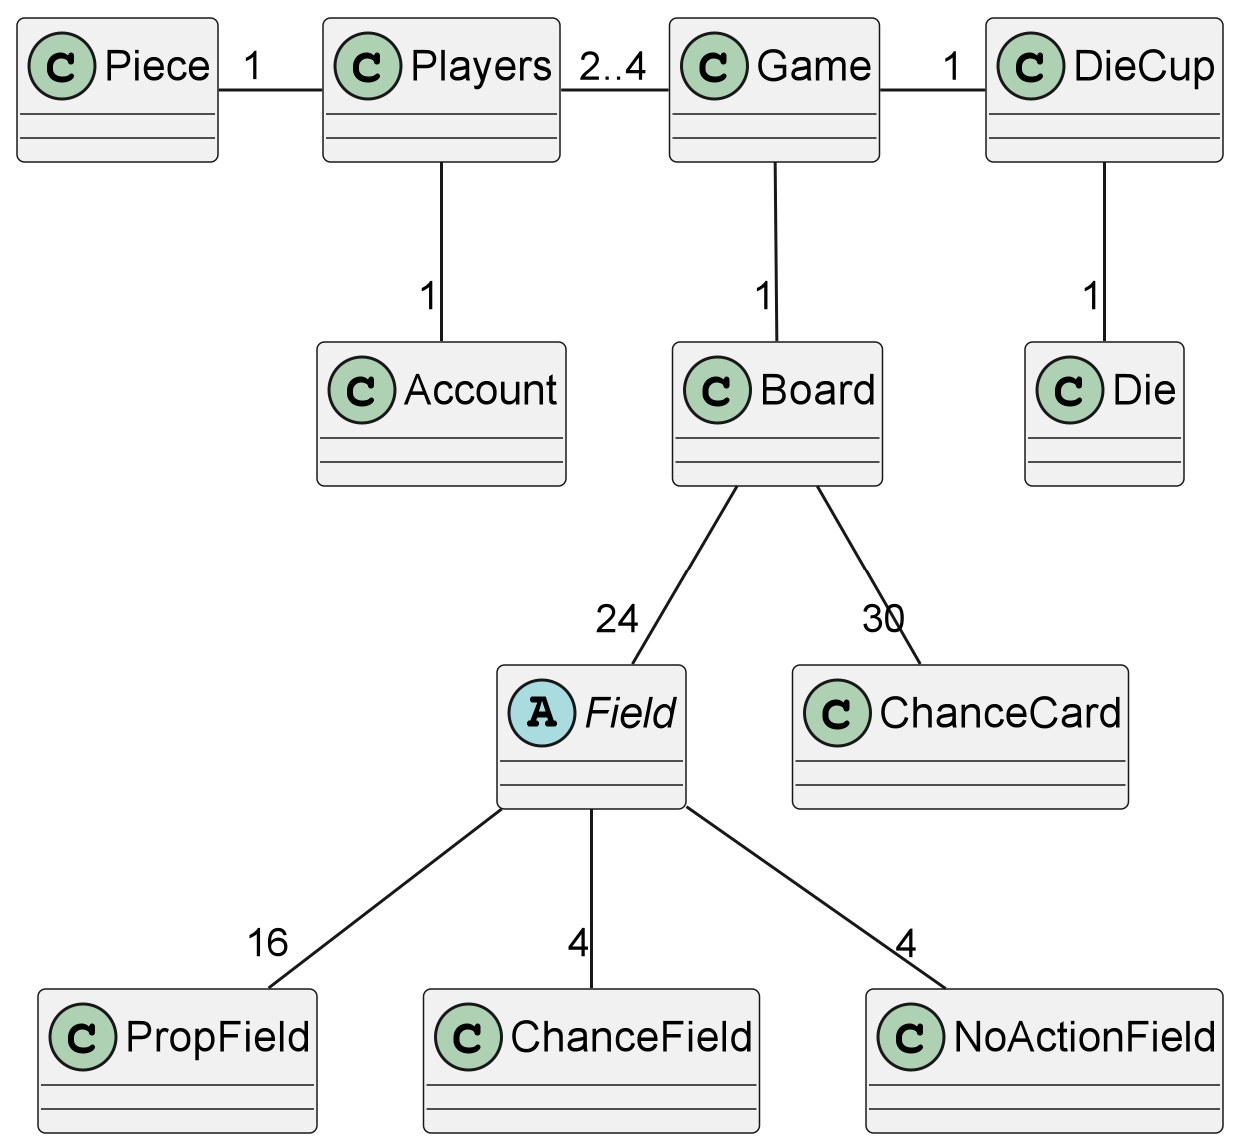
\includegraphics[width = 0.4\textwidth]{Billeder/Domænemodel.png}
    \caption{Domænemodel}
    \label{Domænemodel}
\end{figure}

Vores domænemodel (figur 1) giver os et overblik over hvilke, og hvor mange, elementer der skal være med i vores spil, og hvilken sammenhæng de har. De forskellige delelementer i domænemoddellen er reelle objekter vi vil have med i vores spil, og de danner inspirationsgrundlag til vores design klasse diagram hvor vi kan lave en næsten direkte overførsel fra 'virkelige objekter' til klasser.

\section{Design}
For at give os selv et overblik over spillet, hvordan vores domæne skal se ud, hvilke klasser vi vil implementere og, hvordan system og aktør skal interagere med hinanden, har vi lavet følgende diagrammer.
\\

\begin{figure} [h]
    \centering
    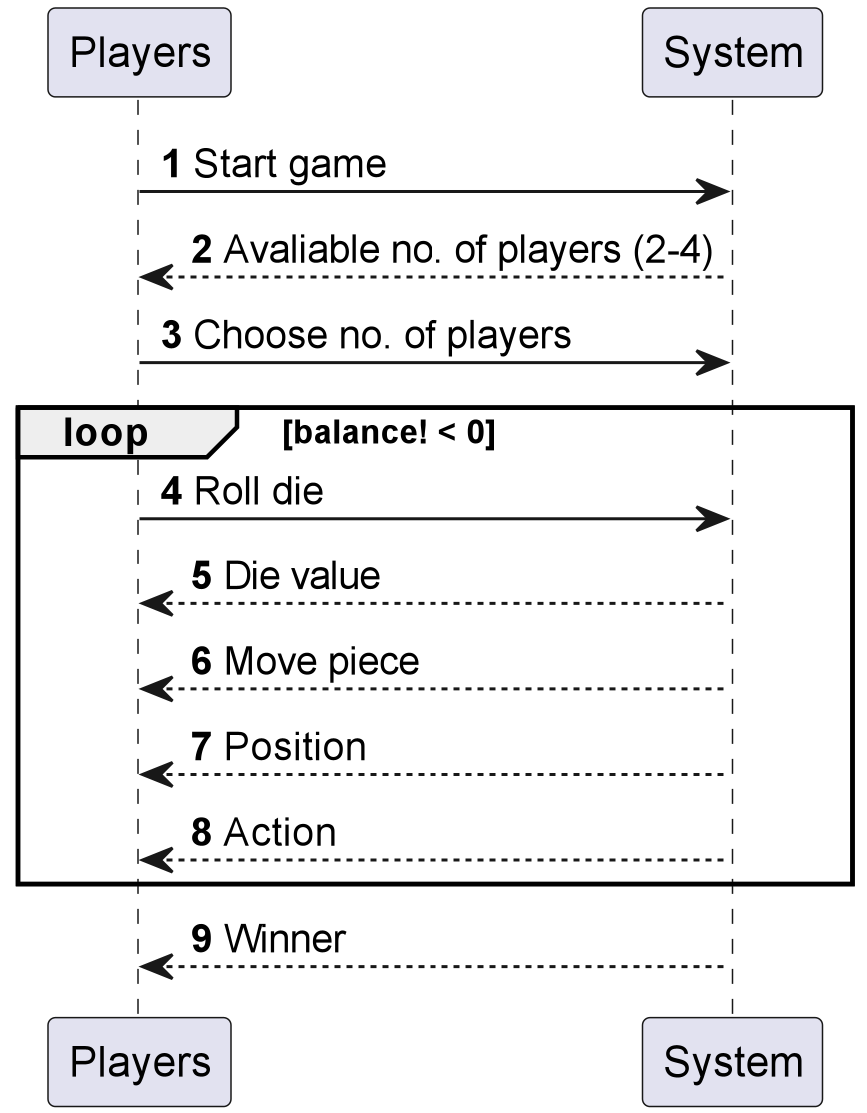
\includegraphics[width = 0.4\textwidth]{Billeder/Systemsekvensdiagram.png}
    \caption{Systemsekvensdiagram}
    \label{Systemsekvensdiagram}
\end{figure}
Vores system sekvens diagram (Figur 4) illustrerer, interaktionen mellem spiller og system igennem en hel iteration spillet. Diagrammet illustrerer at man kun skal starte spillet, vælge antal spillere og slå terning, resten gør system, som giver bedskeder tilbage til spilleren om hvad man har slået, hvor man rykker hen og hvilket feltet man lander på gør. Dette loop fortsætter indtil en spillers pengebeholdning går i nul, og en vinder bliver valgt.  Diagrammet giver  tilmed inspirationsgrundlag til design sekvensdiagrammet hvor metoder bliver tilføjet.   
\\

\begin{figure} [h]
    \centering
    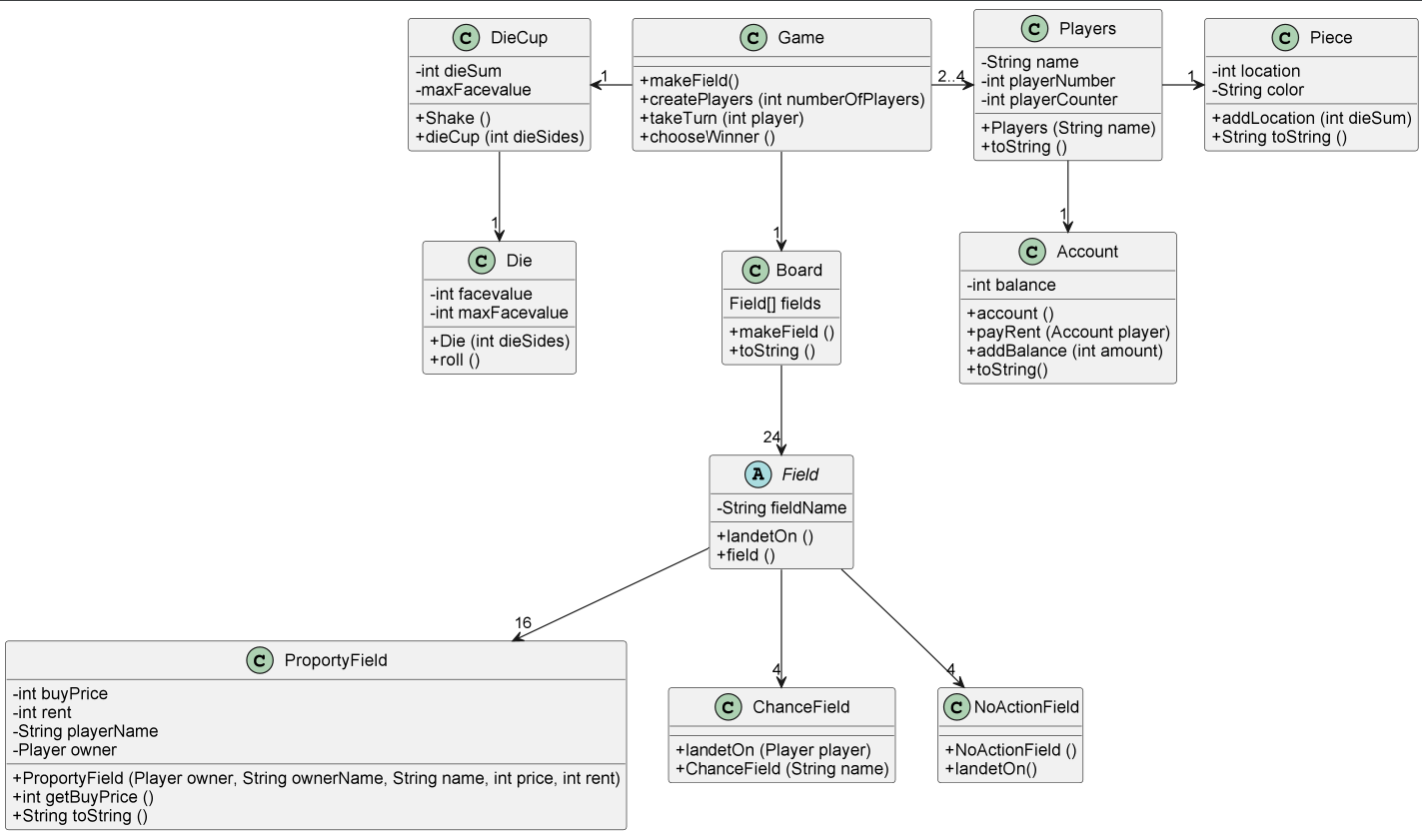
\includegraphics[width = 1.0\textwidth]{Billeder/DesignKlasseDiagram.png}
    \caption{Designklassediagram}
    \label{Designklassediagram}
\end{figure}

Designklasse diagrammet er bygget på vores domænemodel, hvor vi har overført vores delelementer til klasser.  Vores 'player' klasse opretter instanser af account og piece (Creator), hvori account klassens ansvar er at holde holde den specifikke spillers pengebeholdning og piece klassen har ansvaret for at holde spillerens placering (information expert).
Vi har også valgt at lave en abstract class, 'field', som er super-klassen til de 3 polymorfiske underklasser: propertyfield, chancefield, og nonactionfield. De 3 underklasser arver attributter og metoden landedOn() fra superklassen. Vi har valgt at gøre field-klassen abstract og dens underklasser polymorfiske da underklassen deler nogle attributter, i form af at de alle er felter, men de kan nogle forskellige ting, som bliver udført igennem landendOn metoden. Resultatet af dette, er at vi kan lave et enktelt array i vores board-klasse der indeholder alle vores felteobjekter.
Vores game-klasse er vores game-controller, der allokerer ansvaret for input-events til de forskelige klasser (controller) og videre ud til spilleren, igennem GUI-controlleren og til sidst GUI'en.
\\
\\
\begin{figure} [h]
    \centering
    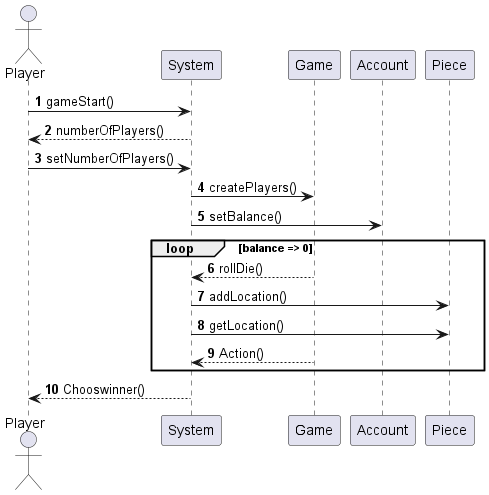
\includegraphics[width = 0.6\textwidth]{Billeder/DesignSequenceDiagram.png}
    \caption{Designsekvensdiagram}
    \label{Designsekvensdiagram}
\end{figure}
\\
Dette designsekvensdiagram(Figur 5) viser hvordan ,og i hvilken rækkefølge, de forskellige klasser snakker sammen. Det kan ses at en  spillers balance bliver givet til en klasse Account og har dermed ansvaret for spillernes pengesum eller balance. Derudover kan det også ses at alle Locations metoderne bliver udført i klasse Piece, da det er information expert. 
\\
\\
\section{Dokumentation}
Når man bruger og har fokus på objekt orienteret programmering, skal man lave instansser af klasserne, hvor de herfra kan arve fra hinanden. En subklasse arver attributter og metoder fra en anden klasse, hvor denne klasse bliver til en superklasse. Man vil derfor lave et klassehierarki, hvor subklasserne arver fra superklasserne. 
\\
\\
En abstrakt klasse er en klasse, der i sig selv ikke kan instansieres, men bruges derimod som superklasse, hvor sub-klasser kan arve attributter og metoder fra den. Man har polymorfiske sub-klasser der deler nogle attributter og metode(r), men skal kunne forskellige ting. Dette har vi brugt i tilfældet for vores abstract super-klasse 'field' og dens sub-klasser (de tidligere nævnte field-klasser).
\\
\\
Hvis en fieldklasse har en landOnField metode, hvor alle subklasserne bruger denne metode, bliver fieldklassen derfor til en abstrakt klasse. 

\subsection{Konfigurationsstyring}
\subsubsection{Udviklingsplatform}
\begin{itemize}
    \item [\textbf{Operativsystem}] Windows 10+, macOS Venturra
    \item [\textbf{java}] Version 8 update 351 (build 1.8.0\_351-b10)
    \item [\textbf{IDE}] IntelliJ IDEA 2022.2.3 (Ultimate Edition)\\
    Build \#IU-222.4345.14, built on October 5, 2022
    \item[\textbf{Libraries}] Matador GUI: \href{https://github.com/diplomit-dtu/MatadorGUIGuide/tree/3.2.x}{https://github.com/diplomit-dtu/MatadorGUIGuide/tree/3.2.x}

 \subsubsection{Dokumentation} Vores artifakter samt dokumentation bliver versionsstyret gennem Git og samles i et GitHub-repo. Den nyeste version af disse vil derfor findes i branchen "Development" og helt færdige produkter vil ligger i "Master".\\
    Rapport og dokumentation bliver samlet i Overleaf som pusher til et repo. Artifakter bliver produceret og redigeret i IntelliJ ved brug af PlantUML og er også versionsstyret med git og pushes til Github.
\end{itemize}

\section{Implementering}
Vi har forsøgt at implementere de klasser, der ifølge vores klassediagram er længst ude i forgreninger og samtidig også har færrest associationer til andre klasser.

\section{Test}
\subsection{Test case 01}
\begin{tabular}{ | m{0.2\textwidth} | m{0.8\textwidth}|}
    \hline
    Test case ID & TC01  \\
    \hline
    Summary & Tester at det rigtige antal spillere er indlæst fra brugeren, oprettet i spillet, oprettet som brikker, oprettet som pengebeholdning og vist til spilleren.\\
    \hline
    Requirements & Tester ift. krav 1, 4 og 7.\\
    \hline
    Preconditions & En bruger starter spillet.\\
    \hline
    Postconditions & Brugerne kan se deres brikker på skærmen og skal begynde at slå med terning.\\
    \hline
    Test Procedure & \begin{enumerate}[itemsep=0.1mm]
        \item Vælg antal spillere
        \item Indtast navne på spillere
        \item Tjek at der vises netop det antal brikker der matcher antal spillere
        \item Tjek at navnene på spillerne matcher det der blev indtastet
    \end{enumerate}\\
    \hline
    Test data &  Spillere = 4\\
     & Spillernavne = TestPerson1, TøstPærsån2, TestPersonMedMegetLangtNavn, (og en kun med mellemrum)\\
    \hline
    Expected result & Det ønskede antal brikker bliver vist til spillerne med de rette navne tilhørende.\\
    \hline
    Actual result & Længere navne bliver skåret korte af felterne på brættet. Ikke ideelt, men indlæsningen fungere og man kan umiddelbart se navnene og brikker.\\
     & 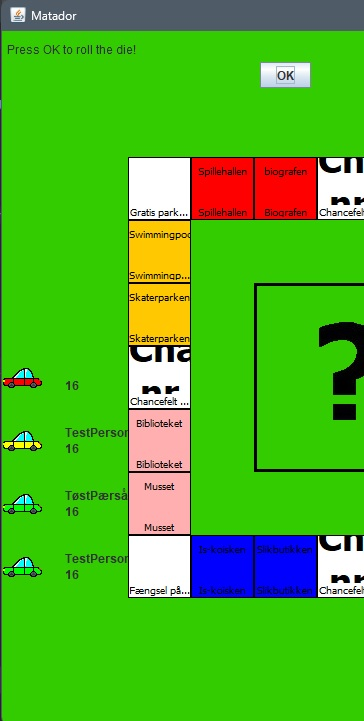
\includegraphics[height = 10cm]{Billeder/TC01.jpg}\\
    \hline
    Status & Gennemført.\\
    \hline
    Tested by & Jakob Agergaard\\
    \hline
    Date & 18-11-2022\\
    \hline
    Test environment & IntelliJ IDEA 2022.2.3 (Ultimate Edition)\\
      & Build \#IU-222.4345.14, built on October 5, 2022\\
      & on Windows 11 Home version 22H2\\
    \hline
\end{tabular}
\subsection{Test case 02}
\begin{tabular}{ | m{0.2\textwidth} | m{0.8\textwidth}|}
    \hline
    Test case ID & TC02  \\
    \hline
    Summary & Tester om spillerne kan udføre en tur\\
    \hline
    Requirements & Tester ift. krav 3, 6 og 7.\\
    \hline
    Preconditions & Bruger har indtastet antal spillere og navne.\\
    \hline
    Postconditions & Turen gives videre til næste spiller (loop fortsætter)\\
    \hline
    Test Procedure & \begin{enumerate}[itemsep=0.1mm]
        \item Tryk enter/OK for at slå med terningen
        \item Tryk enter/OK for at flytte brikken
        \item Tryk enter/OK for at anerkende besked fra system
        \item Tryk enter/OK for at give turen videre
        \item Gentag ovenstående mindst 4 gange
    \end{enumerate}\\
    \hline
    Test data & Manuelt input gennem GUI (Tryk OK, for at spillet går til næste stadie)\\
    \hline
    Expected result & Systemet kører spillerens tur igennem og meddeler derefter hvilken spiller der nu skal til at tage sin tur.\\
    \hline
    Actual result & Der opstår en NullPointerError i linje 78 Der forsøger at opdatere spillerens balance i GUI'en. Den samme fejl vil formentlig også vise sig i linje 79.\\
     & 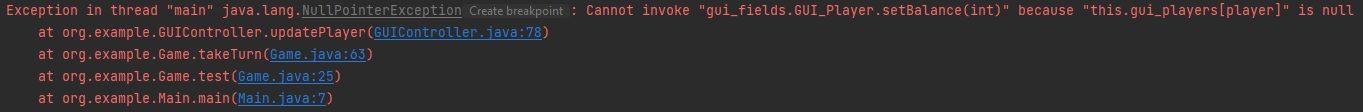
\includegraphics[width = 0.8\textwidth]{Billeder/TC02-1.jpg}\\
     & 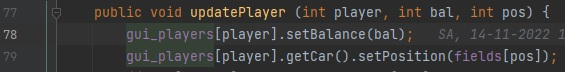
\includegraphics[width = 0.6\textwidth]{Billeder/TC02-2.jpg}\\
     & Ved nærmere undersøgelse fandt vi ud af hvorfor dette skete. Grunden findes i metoden der opretter netop gui\_players arrayet.\\
     & 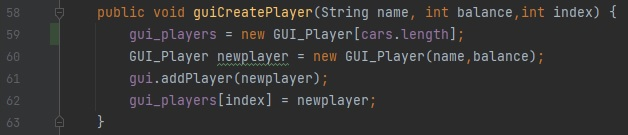
\includegraphics[width = 0.6\textwidth]{Billeder/TC02-3.jpg}\\
     & Løsningen på dette blev at lade dette array blive oprettet allerede umiddelbart efter spillernes brikker er blevet oprettet\\
     & 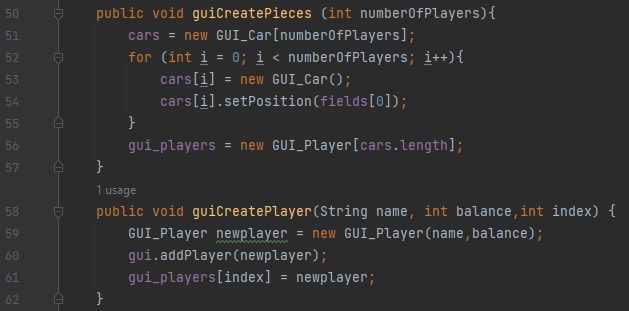
\includegraphics[width = 0.6\textwidth]{Billeder/TC02-4.jpg}\\
    \hline
    Status & Først fejlet.\\
     & Efterfølgende fikset og gennemført.\\
    \hline
    Tested by & Jakob Agergaard\\
    \hline
    Date & 18-11-2022\\
    \hline
    Test environment & IntelliJ IDEA 2022.2.3 (Ultimate Edition)\\
      & Build \#IU-222.4345.14, built on October 5, 2022\\
      & on windows 11 Home version 22H2\\
    \hline
\end{tabular}
\subsection{Brugervenlighed}
\\
\begin{tabular}{ | m{0.2\textwidth} | m{0.8\textwidth}|}
    \hline
    Test case ID & TC03  \\
    \hline
    Summary & Brugertest af 2 -og 3 personer. Testen bliver udført i to omgange. \\
    \hline
    Requirements & Testpersonerne skal kunne læse og anvende keyboard/mus.\\
    \hline
    Preconditions & De har fået spillet opstartet, simple instrukser samt spillets regler.\\
    \hline
    Postconditions & At spillerne ikke gider at gennemføre spillet grundet programmets brugervenlighed.\\
    \hline
    Test Procedure & \begin{enumerate}[itemsep=0.1mm]
        \item Angiv antal spillere 
        \item Skriv navne på spillere 
        \item Tryk enter/OK for at slå med terningen
        \item Tryk enter/OK for at flytte brikken
        \item Tryk enter/OK for at anerkende besked fra system
        \item Tryk enter/OK for at give turen videre
    \end{enumerate} \\

    \hline
    Expected result & At spillet gennemføres og en vinder findes. \\
    \hline
    Actual result & Spillet blev gennemført, dog med visse overvejelser/observationer, med programmets begrænsninger og simplicitet taget i betragtning. Testpersonernes feedback: \begin{enumerate}[itemsep=0.1mm]
        \item Grammatisk fejl, det hedder dice og ikke die. 
        \item Når man bliver informeret om at man er kommet i fængsel, er man ikke kommet i fængsel. 
        \item I stedet for at skulle trykke "OK" vil de have en timer på teksten, så man er "tvunget" til at læse teksten, ellers er det for meget op til en selv, også trykker man for hurtigt, og går glip af vigtig info i spillet. 
    \end{enumerate}\\
    \hline
    Status & Spillet er gennemført uden problemer der har afgørende effekt på programmet\\
    \hline
    Tested by & 3 vilkårlige personer. Testpersonerne er i aldersgruppen 19-25 år. Testpersonerne er både Mænd og Kvinder.\\
    \hline
    Date & 24-11-2022\\
    \hline
    Test environment & IntelliJ IDEA 2022.2.3 (Ultimate Edition)\\
    &Mac OS Ventura\\
    \hline
\end{tabular}
\subsection{JUnit Tests}
Vi har lavet to Unit-tests, men vi ville gerne have lavet flere. Vi oplevede problemer da vi ville lave tests der testede om inputtet fra brugeren blev brugt korrekt.
\begin{figure} [h]
    \centering
    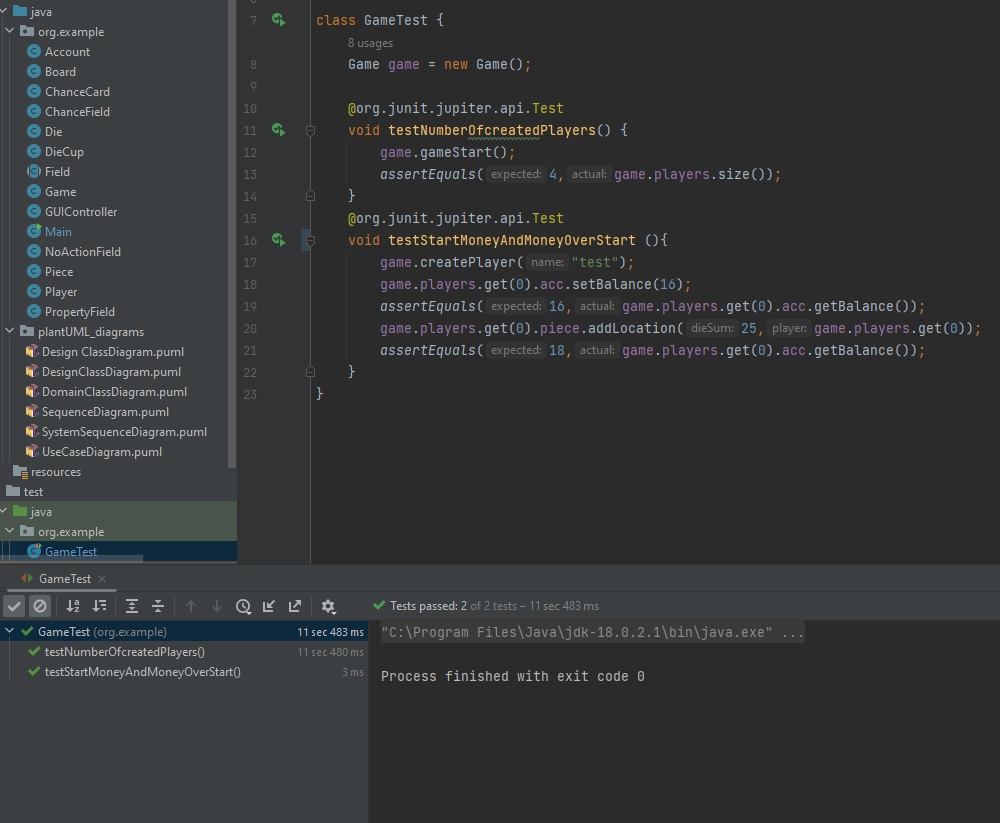
\includegraphics[width = \textwidth]{Billeder/UnitTests.jpg}
    \caption{Fuldførte Unit-tests}
    \label{fig:my_label}
\end{figure}
\subsection{Bugs identificeret}
\begin{itemize}
\item \textbf{(Fjernet)} I implementeringen af chancekortene, stødte vi på et problem der gjorde at, når der landes på et chancefelt, så vises ét chancekort, men handlingerne for et andet chancekort bliver udført\\
Årsagen til dette var at der, når man lander på et 					chancekort, bliver valgt tilfældigt mellem tre mulige chancekort-handlinger, og denne bliver derefter udført. På samme måde blev tekst for chancekortet (displayChanceCard(txt)), også valgt tilfældigt mellem tre mulige chancekort-handlinger. \\
Disse var altså uafhængige af hinanden, og derfor opstod problemet.
Vi endte med at udelade brugen af displayChanceCard(txt), og vores chancekort bliver derfor heller ikke vist når man trækker dem.

\item En bug er, hvis man er to personer, som hedder det samme, og skriver det samme navn ind to gange til systemet, så vil systemet se det som en spiller.

\item  En bug er, man betaler først rent til modstanderen runden efter sin egen. 

\item En bug er at en spilleres balance kan godt være negativ, og spillet vil stadig fortsætte. Hvis den første spiller går i minus, så vil runden spilles færdig, så hvis en modstander lander på en af hans grunde, så vil han få rent og derfor ikke længere være i minus. Spillet burde spillet lige så snart at en af spillerenes balance går i minus, da man har tabt lige så snart man går  i minus

\item \textbf{(Løst)} En bug er, man køber ikke det felt man lander på efter man har trukket et chancekort. 
\\
Problemet var at chancekortene kun kørte ’set-loaction’ metoden, som ikke også kører 'landedOn' metoden. Løsningen til dette var at ændre chancekortene, så de ikke bruger 'set-location' metoden, men kun 'add-location' metoden, som også derefter kører 'landedOn' metoden. Efter denne ændring virkede chancekortene som det var meningen.
\end{itemize}

\section{Konklusion}
På baggrund af kundens vision, vores funktionelle kravliste og vores liste af regler vi løbende ville implementere i prioriteret rækkefølge, kan vi konkludere at vi har lavet et spil, der opfylder de funktionelle krav, samt størstedelen af  de regler vi ville implementere. Dog har vi hverken prioriteret eller implementeret, en funktion for let at kunne oversætte spillet til et andet sprog da: 1. Opgaven var umiddelbart uoverskuelig og 2. Vi mente det var vigtigere at lave et spil der faktisk virkede end et ikke-eksisterende spil, der kunne oversættes til swahili.
\\
\section{Bilag}
\subsection{Litteratur}
\subsection{Kode}
Koden til projektet findes i følgende repository på Github: \href{https://github.com/Jakob-SA/CDIO-}{https://github.com/Jakob-SA/CDIO-3}


\end{document}